% Author: Andrej Binovsky <xbinov00@stud.fit.vutbr.cz>
% Author: Zdenek Lapes <xlapes02@stud.fit.vutbr.cz>
% Author: Andrei Shchapaniak <xshcha00@stud.fit.vutbr.cz>
% Author: Richard Gajdosik <xgajdo33@stud.fit.vutbr.cz>


\documentclass[a4paper, 11pt]{article}


\usepackage[slovak]{babel}
\usepackage[utf8]{inputenc}
\usepackage[left=2cm, top=3cm, text={17cm, 24cm}]{geometry}
\usepackage{times}
\usepackage{verbatim}
\usepackage{enumitem}
\usepackage{graphicx} % vkladanie obrazkov
\usepackage[unicode]{hyperref}
\hypersetup{
    colorlinks = false,
    hypertexnames = false,
}

\newcommand{\RNum}[1]{\uppercase\expandafter{\romannumeral #1\relax}} % makro na sázení římských čísel

%%%%%%%%%%%%%%%%%%%%%%%%%%%%%%%% Andrei import -- LL tabulka/pravidla %%%%%%%%%%%%%%%%%%%%%%%%%%%%%%%%

\usepackage{xcolor}
\usepackage{float}
\usepackage{listings}
\usepackage{amsmath}
\usepackage{bm}
\usepackage{makecell}
\usepackage{cprotect}
\usepackage{multirow}
\usepackage{array}
\usepackage{changepage}
\usepackage{color, colortbl}
\definecolor{LightCyan}{rgb}{0.88,1,1}
\definecolor{White}{rgb}{255,255,255}

\def\nonterm #1{\boldmath{$<$}\textbf{#1}\boldmath{$>$}\space}
\def\rot #1{{\rotatebox[origin=c]{90}{\term{#1}}}}
\def\term #1{\texttt{#1}\space}
\newcommand{\arrow} {$\color{red} \rightarrow$\space}
\newcommand{\unsc} {\underline{\hspace{0.2cm}}}
\newcolumntype{P}[1]{>{\centering\arraybackslash}p{#1}}


%%%%%%%%%%%%%%%%%%%%%%%%%%%%%%%% Andrei import -- LL tabulka/pravidla %%%%%%%%%%%%%%%%%%%%%%%%%%%%%%%%

\begin{document}


    %%%%%%%%%%%%%%%%%%%%%%%%%%%%%%%% Titulná stránka %%%%%%%%%%%%%%%%%%%%%%%%%%%%%%%%
    \begin{titlepage}
        \begin{center}
            
\includegraphics[width=0.77\linewidth]{src/FIT_logo.pdf} \\

            \vspace{\stretch{0.382}}

            \Huge{Projektová dokumentácia} \\
            \LARGE{\textbf{Implementácia prekladača imperatívneho jazyka IFJ21}} \\
            \Large{Tým 082, varianta \RNum{2}}
            \vspace{\stretch{0.618}}
        \end{center}

        \begin{minipage}{0.4 \textwidth}
        {\Large \today}
        \end{minipage}
        \hfill
        \begin{minipage}[r]{0.6 \textwidth}
            \Large
            \begin{tabular}{l l l}
                \textbf{Andrei Shchapaniak} & \textbf{(xshcha00)} & \quad 25\,\% \\
                Andrej Binovsky & (xbinov00) & \quad 25\,\% \\
                Zdenek Lapes & (xlapes02) & \quad 25\,\% \\
                Richard Gajdosik & (xgajdo33) & \quad 25\,\% \\
            \end{tabular}
        \end{minipage}
    \end{titlepage}



    %%%%%%%%%%%%%%%%%%%%%%%%%%%%%%%% Obsah %%%%%%%%%%%%%%%%%%%%%%%%%%%%%%%%
    \pagenumbering{roman}
    \setcounter{page}{1}
    \tableofcontents
    \clearpage



    %%%%%%%%%%%%%%%%%%%%%%%%%%%%%%%% Úvod %%%%%%%%%%%%%%%%%%%%%%%%%%%%%%%%
    \pagenumbering{arabic}
    \setcounter{page}{1}

    \section{Úvod}
    Cieľom projektu bolo vytvoriť funkčný prekladač napísaný v jazyku \texttt{C}, ktorý bude prekladať zdrojové kódy jazyka
    \texttt{Teal} do cielového jazyka \texttt{IFJcode21}, ktorý následne spracováva internet.
    Program musí prijímať zdrojový program zo štandardného vstupu a vypisovať skompilovaný program na štandardný výstup.




    %%%%%%%%%%%%%%%%%%%%%%%%%%%%%%%% Návrh a implementace %%%%%%%%%%%%%%%%%%%%%%%%%%%%%%%%
    \section{Návrh a~implementácia}

    \subsection{Lexikálna analýza}
    \texttt{Scanner} slúži pre lexikálnu analýzu. Je implementovaný ako deterministický konečný automat, ktorý rozpoznáva všetky
    prichádzajúce tokeny. Uchováva informácie o tom či sa jedná o komentár, identifikátor, textové bloky, relačné
    operátory alebo iné validné, poprípade nevalidné tokeny u ktorých nastane lexikálna chyba 1. V~prípade validného
    tokenu na základe koncového stavu sa vyplnia nasledujúce informácie v štruktúre \texttt{token\_t}:
    \begin{itemize}
        \item \texttt{type}  --  typ načítaného tokenu
        \item \texttt{keyword} -- keď typ je \texttt{T\_KEYWORD}, do premennej keyword sa uloží odpovedajúca hodnota
        \item \texttt{attr.num\_i} -- číslo \texttt{integer}d
        \item \texttt{attr.num\_f} -- číslo \texttt{double}
        \item \texttt{attr.id} -- ostatné tokeny
    \end{itemize}
    V prípade že sa narazí na blok, ktorý označuje komentár je časť kódu ignorovaná a lexikálna analýza pokračuje
    až dalším tokenom mimo spomenutý blok.

    \subsection{Syntaktická analýza}
    Parser je hlavným modulom prekladača, protože komunikuje se všetkými ostatnými modulmi a riadi celú funkčnosť
    prekladača. Syntaktická analýza sa vykonáva zhora dolu metódou rekurzivného zostupu.
    Syntaktická analýza dostáva postupne od lexikálneho analyzátoru tokeny, ktoré následne musia spĺňať presnú
    syntaktickú štruktúru a postupnosť podla pravidiel \texttt{LL-gramatiky}.
    V prípade porušenia pravidla (typ prichádzajúceho tokenu se líší od očakávaného) sa vyhodí syntaktická chyba 2.
    V priebehu syntaktickej analýzy sú volané funkcie z modulu pre generovanie kódu, ktoré vygenerujú cielový kód z
    jazyka \texttt{Teal} do \texttt{IFJcode21}, ktorý nasledné spracováva interpret.


    \subsection{Spracovanie výrazov pomocou precedenčnej syntaktickej analýzy}
    Precedenčná syntaktická analýza je modul ktorý zaisťuje spracovanie výrazov metódou zdola hore.
    Vo svojom rozhraní obsahuje \texttt{expr()}, ktorú volá parser, keď chce precedenčnej analýze predať
    riadenie vo chvíli, kedy očakáva výraz.
    \subsubsection{Implementácia precedenčnej tabuľky}
    Postupne precedenčná analýza spracováva tokeny a pomocou precedenčnej tabuľky symbolov
    určuje precedenciu. Na základe tejto precedencie môže nastať päť stavov:
    \begin{enumerate}
        \item Pri precedencii \texttt{<} pridávame na zásobník načítaný token spolu so znakom precedencie.
        \item Pri precedencii \texttt{>} redukujeme dva výrazy na jeden a ukladáme ich typ podľa pravidla.
        \item Pri precedencii \texttt{=} zapíšeme načítaný znak z tokenu na zásobník.
        \item Pri precedencii \texttt{e} sme narazili na nesprávne poradie znakov a nastáva sémantická chyba.
        \item Pri precedencii \texttt{s} sme narazili na dva identifikátory alebo znak '\texttt{)}' a identifikátor. Následne redukujeme zvyšok výrazu a vraciame parseru riadenie.
        \item Pri precedencii \texttt{s} sme narazili na dva identifikátory alebo znak '\texttt{)}' a identifikátor. Následne redukujeme zvyšok výrazu a vraciame parseru riadenie.
    \end{enumerate}
    \subsection{Sémantická analýza}

        Sémantické chyby pre nekompatibilitu typu priradenia, návratových hodnôt a predaných
        argumentov do funkcií sa detekujú pomocou dvoch polí \texttt{tps\_left} a \texttt{tps\_right}. Po spracovaní
        určitého pravidla sa vykoná porovnanie podľa sémantiky jazyka \texttt{IFJ21}.
        Kompatibilita typu vo výraze sa detekuje tým istým spôsobom s rozdielom použitia dvoch premenných typu \texttt{char}.
        Sémantické chyby pre nedefiníciu, redefiníciu sa detekujú pomocou tabuliek symbolov. Globálna tabulka
        symbolov je určená pre názvy funkcií. Pre názvy premenných je vytvorený zásobník
        tabuliek symbolov. Dôvodom implementácie zásobníka je riešenie problému s totožnými názvami premenných v
        rôznych rámcoch.



    \subsection{Generovanie cielového kódu}
    Generovanie cieľového kódu \texttt{IFJcode21} je implementovaný ako samostatný modul, ktorý je riadený syntaxou.
    Komponenty modulu sú volané v parseri na základe pravidiel \texttt{LL-gramatiky}. Z dôvodu neoptimalizácie sa cieľový kód
    generuje priamo bez tvorby trojadresného kódu.

    \subsubsection{Implementácia výpisu cieľového kódu}
    Na zaistenie výpisu cieľového kódu len za podmienky bezchybnej analýzy zapisujeme cieľový kód do dvoch textových
    blokov -- definície funkcií a volanie funkcií. Tieto dva textové bloky po úspešnej analýze\\ skonkatenujeme a
    vypíšeme na štandardný výstup.

    \subsubsection{Generovanie -- deklarácie premenných}
    Deklarácie premenných a ich možný konflikt názvov (na základe výskytu toho istého názvu v rôznych rámcoch)
    sme implementovali vďaka obojsmernému radu v ktorom sa ukladá adresa elementu tabulky
    symbolov s príslušným identifikátorom. Element tabulky obsahuje unikátne číslo premennej, ktorý zaisťuje jedinečnosť
    názvu premennej.

    \subsubsection{Generovanie -- funkcie}
    Volanie funkcií je zaistené vygenerovaním kódu, ktorý predá funkcii argumenty pomocou dočasného rámcu. Následne
    je vygenerovaný kód pre zavolanie funkcie. Pre správnu funkčnosť volanej funkcie je ihneď na začiatku generovaný kód,
    ktorý z dočasného rámca vytvori lokálny rámec funkcie a pre všetky argumenty ktoré boli funkcii predané vytvori
    promenné s názvami podľa parametrov funkcie. Následne sa generuje kód tela funkcie.

    \subsubsection{Generovanie -- výrazy}
    Generovanie kódu pre výraz sa začne vykonávať ihned po jeho redukcii. V priebehu redukcii je výraz zapísaný do obojstranného radu
    v postfixovom formáte. Jednotlivé elementy v rade nesú všetky potrebné
    informácie na generovanie výrazu - typ operátora, názov premennej či hodnotu konštanty. Generátor generuje len inštrukcie
    kódu \texttt{Ifjcode21} ktoré využívajú zásobník. To znamená že hodnoty, medzivýsledky a následne výsledok výrazu sú
    uložené na zásobník.

    \subsubsection{Generovanie -- podmienky a cykly}
    Pre generovanie podmienok a cyklov využívame náveštia, ktoré sú taktiež reprezentované unikátnym číslom a
    názvom funkcie kde sa nachádzajú. Na zabránenie redeklarácie premenných sa telo cyklu zapisuje do dvoch rôznych textových
    blokov. Vyskytnuté deklarácie zapisujeme naďalej do bloku definícií funkcií. No zvyšný kód tela cyklu zapisujeme do
    tretieho pomocného textového bloku. Následne po vygenerovaní celého cyklu tieto dva bloky skonkatenujeme.

    \subsection{Prekladový systém}
    \subsubsection{CMake}
    \texttt{CMake} je multiplatformný nástroj na preklad zdrojových kódov. Nástroj sme vybrali na základe preferencií všetkých
    členov tímu. \texttt{CMake} nám predovšetkým pomáhal kompilovať a testovať výsledný program. Pravidlá pre preklad sú napísané v súbore
    \texttt{CMakeLists.txt} a po spustení nastroja \texttt{CMake} je automaticky vygenerovaný súbor \texttt{Makefile}.
    Na testovanie sme používali \texttt{google testy}, ktoré sme prekladali výhradne pomocou \texttt{CMaku}.

    \subsubsection{Skripty}
    Pre účely testovania boli vytvorené shellovské skripty. Jeden rozsiahly skript, ktorý uľahčoval a automatizoval
    testovanie všetkých častí projektu. Taktiež sme vytvorili sript pre preklad projektu a čistenie prebytočných súborov
    vzniknutých v dôsledku kompilácie projektu či testovacích suborov.

    \subsubsection{GNU Make}
    Zo zadania bolo požadované aby odovzdaný projekt obsahoval \texttt{Makefile}, ktorý s príkazom
    \texttt{make} preloží zdrojové súbory projektu a s príkazom \texttt{make clean} zmazal prebytočné súbory vzniknuté v dôsledku kompilácie.
    Tento nástroj nám taktiež pomáhal zabaliť celý projekt do jedného archívu \texttt{zip}.





    %%%%%%%%%%%%%%%%%%%%%%%%%%%%%%%% Speciální algoritmy a datové struktury %%%%%%%%%%%%%%%%%%%%%%%%%%%%%%
    \section{Špeciálne algoritmy a~dátové štruktúry}

    \subsection{Tabuľka s~rozptýlenými položkami}
    Túto dátovú štruktúru sme si zvolili vďaka časovej zložitosti
    (je reprezentovaná medzi \texttt{O(1)} až \texttt{O(n)}). Taktiež nám pomohli znalosti štruktúry z
    predmetov \texttt{IAL} a \texttt{IJC}. Veľkosť tabuľky jsme zvolili 101.
    Ako unikátny kľúč pre prístup k dátam v tabuľke slúži názov premennej alebo funkcie.
    Každý záznam v tabuľke obsahuje informácie o identifikátore. U premenných je uchovávaná aj informácia
    o hĺbke (redefinícia v zanorenejšom rámci kódu). Modul je implementovaný v súboroch
    \texttt{symtable.h} a \texttt{symtable.c}.


    \subsection{Pole rozptýlených tabuliek}
    Táto dátová štruktúra reprezentuje pole ktoré obsahuje tabuľky s~rozptýlenými položkami. Každá tabuľka reprezentuje
    iný logický rámec.
    Modul je implementovaný v súboroch \texttt{symstack.c} a \texttt{symstack.h}

    \subsection{Obojsmerný rad}
    Obojsmerný rad je kombinácia zásobníka a radu. Je možné do neho vkladať aj odoberať dáta z oboch strán.
    Implementovali sme ho ako samostatný modul pre viac častí projektu.
    Je využívaný najmä v generovaní kódu, kde slúži na uchovávanie postfixového výrazu či
    identifikátorov. Taktiež obsahuje informáciách o parametroch, argumentoch a návratových hodnatách funkcií.
    Modul je implementovaný v súboroch \texttt{queue.c} a \texttt{queue.h}.

    \subsection{Obojsmerný zoznam}
    Táto dátová štruktúra je využitá pre spracovávanie výrazu v súbore \texttt{expressions.c}. Taktiež k štruktúre boli
    implementované funkcie pre jej obsluhu. Zložitosť je reprezentovaná ako \texttt{O(n)} pre vyhľadávanie a \texttt{O(1)}
    pre vkladanie na začiatok zoznamu.

    \subsection{Dynamický reťazec}
    Pre uchovanie vygenerovaného kódu počas prekladu a prácu s identifikátormi sme vytvorili štruktúru \texttt{string\_t}.
    Pre obsluhu štruktúry sme vytvorili pomocné funkcie ako alokácia/dealokácia štruktúry,
    odstraňovanie, pridávanie a konkatenácia reťazcov.
    Modul je implementovaný v súboroch \texttt{str.c} a \texttt{str.h}.


    %%%%%%%%%%%%%%%%%%%%%%%%%%%%%%%% Práce v týmu %%%%%%%%%%%%%%%%%%%%%%%%%%%%%%%%
    \section{Práca v~týmu}
    Ihneď pri skladaní tímu sme si všetci uvedomovali, že sa
    očakáva pravidelná a skorá práca na projekte, čo sa nám nakoniec aj podarilo.
    Každý na projekte pracoval vždy s predstihom a darilo sa nam dodržiavať termíny,
    ktoré sme si stanovili.


    \subsubsection{Komunikácia a spôsob práce v tíme}
    Pre komunikáciu sme používali výhradne komunikačnú platformu \texttt{Discord}. Funguje na
    rovnakom princípe ako platforma \texttt{Slack}, ktorá sa používa profesionálne účely.
    Na danej platforme boli vytvorené komunikačné vlákna
    v ktorých boli založené \texttt{TODO} či \texttt{error} listy. Taktiež tam prebiehala bežná komunikácia či hlasové rozhovory s
    možnosťou zdieľania obrazovky, vďaka čomu sme mohli vyriešiť mnoho problémov
    digitálne a tým aj veľmi rýchlo. Avšak aj napriek
    dobrej digitálnej komunikácii sme sa snažili mať čo najviac
    osobných stretnutí.

    \subsubsection{Verzovací systém a vývojové prostredie}
    Ako vývojové prostredie sme využili \texttt{Clion} a \texttt{Vim}. Vývoj prebiehal na platformách \texttt{MacOs}, \texttt{Linux} a \texttt{Windows}. No
    testovanie prebiehalo len na operačnom systému \texttt{Linux}. Ako verzovací systém sme použili \texttt{git} spolu s portálom
    \texttt{GitHub}.

    \subsection{Rozdelenie práce medzi členmi tímu}
    \leavevmode\newline
    \textbf{Andrei:}
    \begin{itemize}
        \item  Lexikálna, sémantická a obecná syntaktická analýza
        \item  Organizácia a kontrola práce nad projektom
        \item  Tabulka symbolov
    \end{itemize}\leavevmode\newline
    \textbf{Richard:}
    \begin{itemize}
        \item  Syntaktická a sémantická analýza pre výrazy
        \item  Precedenčná tabulka
        \item  Prezentácia
    \end{itemize}\leavevmode\newline
    \textbf{Zdenek a Andrej:}
    \begin{itemize}
        \item  Generovanie kódu
        \item  Automatizácia testovania
        \item  Google testy, tvorba testov
        \item  Dokumentácia
    \end{itemize}


    %%%%%%%%%%%%%%%%%%%%%%%%%%%%%%%% Závěr %%%%%%%%%%%%%%%%%%%%%%%%%%%%%%%%
    \section{Záver}
    Projekt bol zadaný začiatkom semestra, ešte skôr, než boli prebraté všetky potrebné znalosti pre
    úspešné splnenie projektu . Boli sme si ale vedomí zložitosti a obsiahlosti projektu,
    a preto sme čerpali informácie aj zo záznamov prednášok z minulých rokov. To nám dalo potrebné informácie do
    štartu projektu a tým sme mohli začať s implementáciou s dostatočne veľkým predstihom.
    Už začiatkom semestra sme mali zostavený tím. Taktiež sme sa dohodli na komunikačných kanáloch a rozdelení práce. Takže s
    komunikáciou neboli žiadne problémy a každý vedel, čo sa od neho očakáva.
    Ak sme mali nejaké nejasnosti so zadaním, tak všetko sme si vyjasnili buď pomocou diskusného fóra alebo
    neoficiálneho komunikačného kanála študentov. V implementácii projektu sme používali sadu testov
    (vlastných aj zdieľaných s kolegami).
    Tieto testy nam veľmi dobre poslúžili na detekovanie chýb a urýchlenie práce nad projektom.
    Projekt bol pre nás veľmi prínosná skúsenosť. Priamo v praxi sme si objasnili veľa problémov ohľadom prekladačov a naučili sme sa ako fungujú.
    Zároveň sme ako tím zvládli pracovať veľmi pekným tempom. Tímová pomoc bola samozrejmosťou.



    %%%%%%%%%%%%%%%%%%%%%%%%%%%%%%%% Citace %%%%%%%%%%%%%%%%%%%%%%%%%%%%%%%%
    \clearpage
    \bibliographystyle{czechiso}
    \renewcommand{\refname}{Literatura}
    \bibliography{dokumentace}



    %%%%%%%%%%%%%%%%%%%%%%%%%%%%%%%% Přílohy %%%%%%%%%%%%%%%%%%%%%%%%%%%%%%%%
    \clearpage


    %%%%%%%%%%%%%%%%%%%%%%%%%%%%%%%% Diagram konečného automatu %%%%%%%%%%%%%%%%%%%%%%%%%%%%%%%%

    \section*{Diagram konečného automatu specifikujúceho lexikálny analyzátor}
    \begin{figure}[!ht]
        \centering
        \vspace{-1.2cm}
        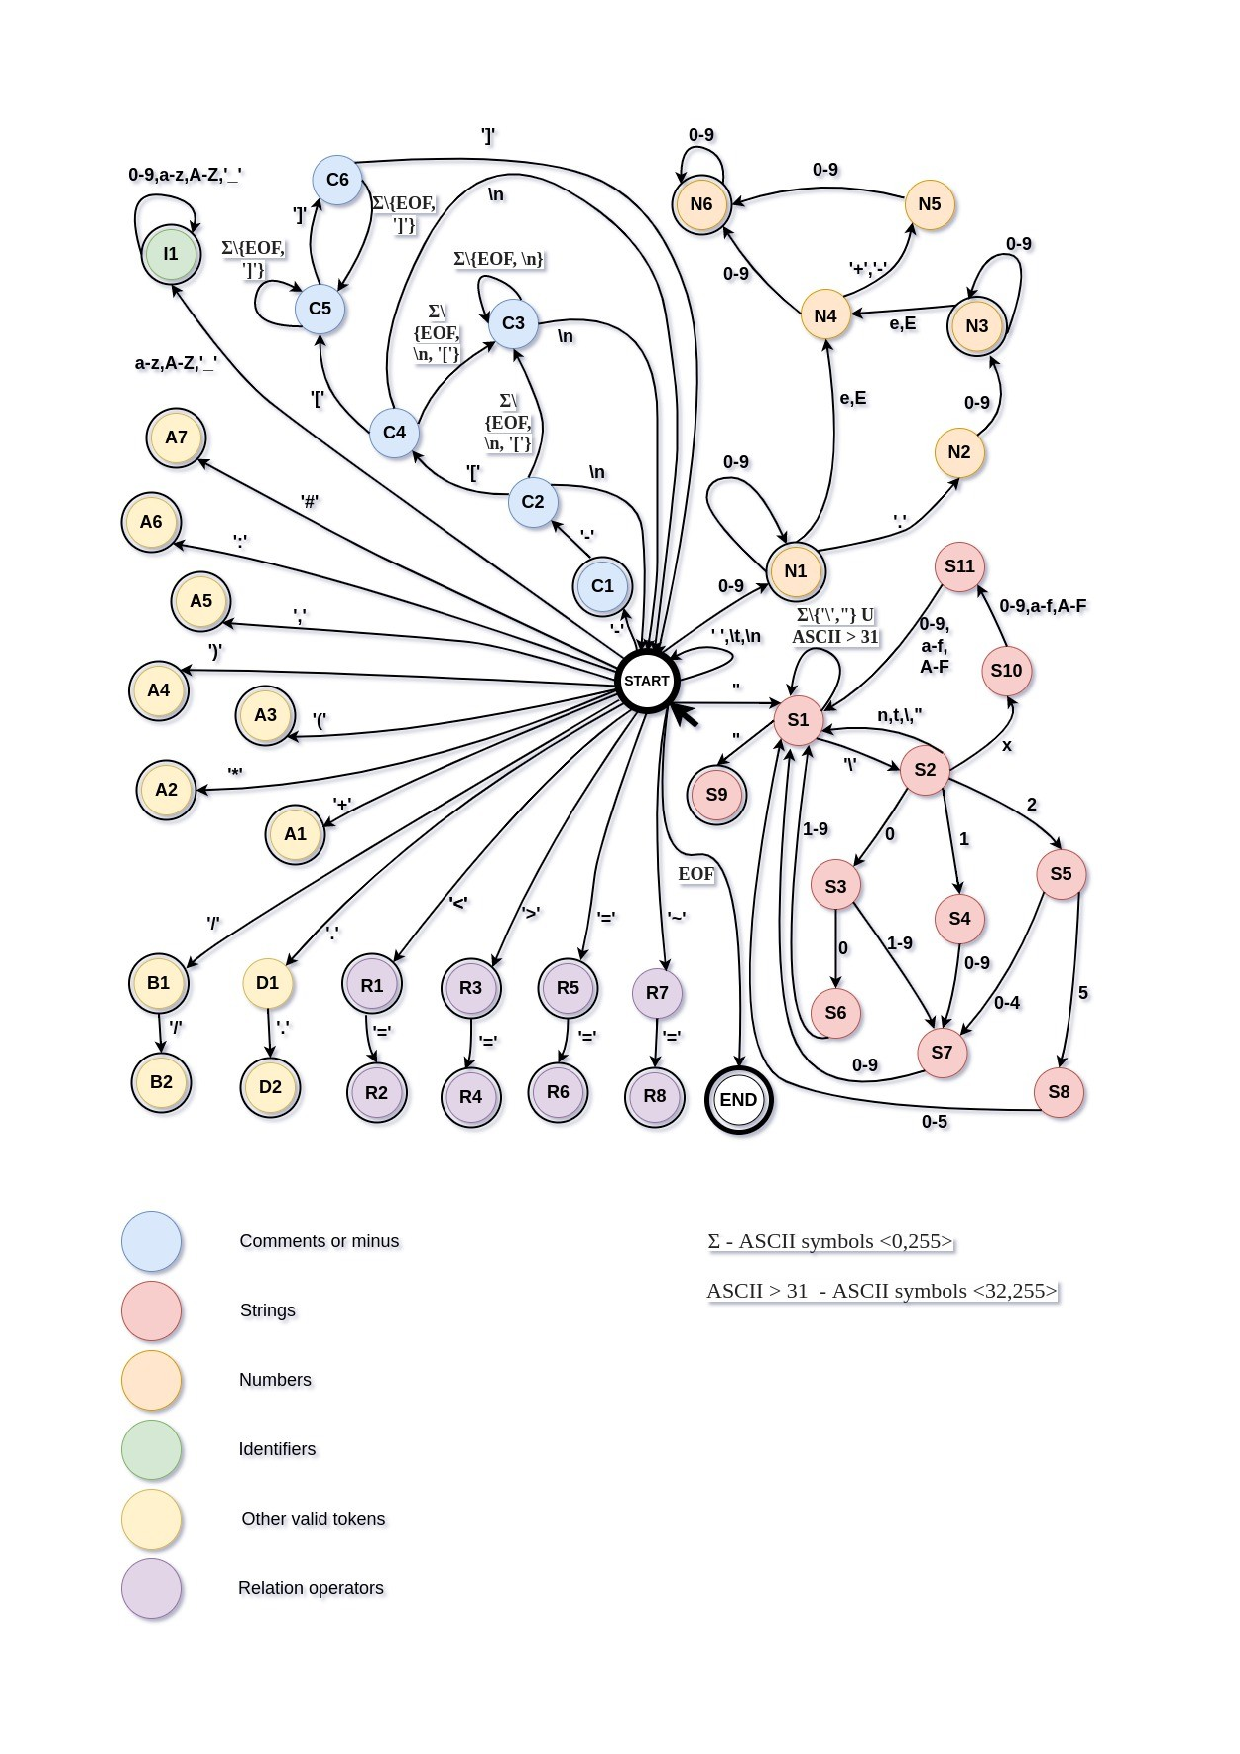
\includegraphics[width=0.95\linewidth]{src/FSM_PDF.pdf}
        \caption{Diagram konečného automatu specifikující lexikální analyzátor}
        \label{figure:fa_graph}
    \end{figure}

    %%%%%%%%%%%%%%%%%%%%%%%%%%%%%%%% LL -- gramatika %%%%%%%%%%%%%%%%%%%%%%%%%%%%%%%%
    \section*{LL -- gramatika}
    \begin{enumerate}[label=\textcolor{red}{\arabic*.}]
        \item \nonterm{prolog} \arrow{} \term{require} \term{t\unsc{}string} \nonterm{prog}

        \item \nonterm{prog} \arrow{} \term{global} \term{id} \term{:} \term{function} \term{(} \nonterm{arg\unsc{}T} \term{)} \nonterm{ret\unsc{}T} \nonterm{prog}

        \item \nonterm{prog} \arrow{} \term{function} \term{id} \term{(} \nonterm{arg} \term{)} \nonterm{ret\unsc{}T} \nonterm{stmt} \term{end} \nonterm{prog}

        \item \nonterm{prog} \arrow{} \term{id} \term{(} \nonterm{param} \term{)} \nonterm{prog}
        \item \nonterm{prog} \arrow{} \term{EOF}

        \item \nonterm{arg\unsc{}T} \arrow{} \nonterm{type} \nonterm{next\unsc{}arg\unsc{}T}
        \item \nonterm{arg\unsc{}T} \arrow{} \term{$\varepsilon$}

        \item \nonterm{next\unsc{}arg\unsc{}T} \arrow{} \term{,} \nonterm{type} \nonterm{next\unsc{}arg\unsc{}T}

        \item \nonterm{next\unsc{}arg\unsc{}T} \arrow{} \term{$\varepsilon$}

        \item \nonterm{ret\unsc{}T} \arrow{} \term{:} \nonterm{type} \nonterm{next\unsc{}ret\unsc{}T}

        \item \nonterm{ret\unsc{}T} \arrow{} \term{$\varepsilon$}

        \item \nonterm{next\unsc{}ret\unsc{}T} \arrow{} \term{,} \nonterm{type} \nonterm{next\unsc{}ret\unsc{}T}

        \item \nonterm{next\unsc{}ret\unsc{}T} \arrow{} \term{$\varepsilon$}

        \item \nonterm{arg} \arrow{} \term{id} \term{:} \nonterm{type} \nonterm{next\unsc{}arg}
        \item \nonterm{arg} \arrow{} \term{$\varepsilon$}

        \item \nonterm{next\unsc{}arg} \arrow{} \term{,} \term{id} \term{:} \nonterm{type} \nonterm{next\unsc{}arg}

        \item \nonterm{next\unsc{}arg} \arrow{} \term{$\varepsilon$}

        \item \nonterm{type} \arrow{} \term{integer}
        \item \nonterm{type} \arrow{} \term{number}
        \item \nonterm{type} \arrow{} \term{string}
        \item \nonterm{type} \arrow{} \term{nil}

        \item \nonterm{stmt} \arrow{} \term{if} \nonterm{expr} \term{then} \nonterm{stmt} \term{else} \nonterm{stmt} \term{end} \nonterm{stmt}

        \item \nonterm{stmt} \arrow{} \term{while} \nonterm{expr} \term{do} \nonterm{stmt} \term{end} \nonterm{stmt}

        \item \nonterm{stmt} \arrow{} \term{local} \term{id} \term{:} \nonterm{type} \nonterm{def\unsc{}var} \nonterm{stmt}

        \item \nonterm{stmt} \arrow{} \term{return} \nonterm{expr} \nonterm{next\unsc{}expr} \nonterm{stmt}

        \item \nonterm{stmt} \arrow{} \term{id} \nonterm{fork\unsc{}id} \nonterm{stmt}

        \item \nonterm{stmt} \arrow{} \term{$\varepsilon$}

        \item \nonterm{def\unsc{}var} \arrow{} \term{=} \nonterm{one\unsc{}assign}
        \item \nonterm{def\unsc{}var} \arrow{} \term{$\varepsilon$}

        \item \nonterm{one\unsc{}assign} \arrow{} \term{id} \term{(} \nonterm{param} \term{)}
        \item \nonterm{one\unsc{}assign} \arrow{} \nonterm{expr}

        \item \nonterm{param} \arrow{} \nonterm{param\unsc{}val} \nonterm{next\unsc{}param}
        \item \nonterm{param} \arrow{} \term{$\varepsilon$}

        \item \nonterm{param\unsc{}val} \arrow{} \term{id}
        \item \nonterm{param\unsc{}val} \arrow{} \nonterm{term}

        \item \nonterm{term} \arrow{} \term{t\unsc{}string}
        \item \nonterm{term} \arrow{} \term{t\unsc{}integer}
        \item \nonterm{term} \arrow{} \term{t\unsc{}number}
        \item \nonterm{term} \arrow{} \term{nil}

        \item \nonterm{next\unsc{}param} \arrow{} \term{,} \nonterm{param\unsc{}val} \nonterm{next\unsc{}param}

        \item \nonterm{next\unsc{}param} \arrow{} \term{$\varepsilon$}

        \item \nonterm{next\unsc{}expr} \arrow{} \term{,} \nonterm{expr} \nonterm{next\unsc{}expr}
        \item \nonterm{next\unsc{}expr} \arrow{} \term{$\varepsilon$}

        \item \nonterm{fork\unsc{}id} \arrow{} \term{(} \nonterm{param} \term{)}
        \item \nonterm{fork\unsc{}id} \arrow{} \nonterm{next\unsc{}id}

        \item \nonterm{next\unsc{}id} \arrow{} \term{,} \term{id} \nonterm{next\unsc{}id}
        \item \nonterm{next\unsc{}id} \arrow{} \term{=} \nonterm{mult\unsc{}assign}

        \item \nonterm{mult\unsc{}assign} \arrow{} \term{id} \term{(} \nonterm{param} \term{)}
        \item \nonterm{mult\unsc{}assign} \arrow{} \nonterm{expr} \nonterm{next\unsc{}expr}
    \end{enumerate}

    %%%%%%%%%%%%%%%%%%%%%%%%%%%%%%%% LL -- tabulka %%%%%%%%%%%%%%%%%%%%%%%%%%%%%%%%
    \newpage
    \section*{LL -- tabulka}

    \begin{table}[htb]
        \begin{adjustwidth}{-0.2cm}{}
            \begin{tabular}{!{\vrule width 2pt}>{\columncolor{LightCyan}}P{2.3cm}!{\vrule width 2pt}P{2.5mm}|P{2.5mm}|P{2.5mm}|P{2.5mm}|P{2.5mm}|P{2.5mm}|P{2.5mm}|P{2.5mm}|P{2.5mm}|P{2.5mm}|P{2.5mm}|P{2.5mm}|P{2.5mm}|P{2.5mm}|P{2.5mm}|P{2.5mm}|P{2.5mm}|P{2.5mm}|P{2.5mm}|P{2.5mm}|P{2.5mm}!{\vrule width 2pt}}
                \Xhline{5\arrayrulewidth} \rowcolor{LightCyan}
                \cellcolor{White}& \rot{require} & \rot{global} & \rot{function} & \rot{id} & \rot{integer}
                & \rot{string} & \rot{number} & \rot{nil} & \rot{t\unsc{}integer} & \rot{t\unsc{number}} & \rot{t\unsc{}string} & \rot{if} & \rot{while} & \rot{local} & \rot{return}  & \rot{:} & \rot{=} & \rot{(} & \rot{,} & \rot{EOF} & \rot{\$}\\
                \Xhline{5\arrayrulewidth}
                \nonterm{prolog} & 1 & & & & & & & & & & & & & & & & & & & & \\
                \hline
                \nonterm{prog} & & 2 & 3 & 4 & & & & & & & & & & & & & & & & 5 &\\
                \hline
                \nonterm{arg\unsc{}T} & & & & & 6 & 6 & 6 & 6 & & & & & & & & & & & & & 7 \\
                \hline
                \nonterm{next\unsc{}arg\unsc{}T} & & & & & & & & & & & & & & & & & & & 8 & & 9 \\
                \hline
                \nonterm{ret\unsc{}T} & & & & & & & & & & & & & & & & 10 & & & & & 11 \\
                \hline
                \nonterm{next\unsc{}ret\unsc{}T} & & & & & & & & & & & & & & & & & & & 12 & & 13 \\
                \hline
                \nonterm{arg} & & & & 14 & & & & & & & & & & & & & & & & & 15 \\
                \hline
                \nonterm{next\unsc{}arg} & & & & & & & & & & & & & & & & & & & 16 & & 17 \\
                \hline
                \nonterm{type} & & & & & 18 & 20 & 19 & 21 & & & & & & & & & & & & &\\
                \hline
                \nonterm{stmt} & & & & 26 & & & & & & & & 22 & 23 & 24 & 25 & & & & & & 27 \\
                \hline
                \nonterm{def\unsc{}var} & & & & & & & & & & & & & & & & & 28 & & & & 29 \\
                \hline
                \nonterm{one\unsc{}assign} & & & & 30 & & & & & & & & & & & & & & & & & 31 \\
                \hline
                \nonterm{param} & & & & 32 & & & & 32 & 32 & 32 & 32 & & & & & & & & & & 33 \\
                \hline
                \nonterm{param\unsc{}val} & & & & 34 & & & & 35 & 35 & 35 & 35 & & & & & & & & & &\\
                \hline
                \nonterm{term} & & & & & & & & 39 & 37 & 38 & 36 & & & & & & & & & &\\
                \hline
                \nonterm{next\unsc{}param} & & & & & & & & & & & & & & & & & & & 40 & & 41 \\
                \hline
                \nonterm{next\unsc{}expr} & & & & & & & & & & & & & & & & & & & 42 & & 43\\
                \hline
                \nonterm{fork\unsc{}id} & & & & & & & & & & & & & & & & & 45 & 44 & 45 & & \\
                \hline
                \nonterm{next\unsc{}id} & & & & & & & & & & & & & & & & & 47 & & 46 & & \\
                \hline
                \nonterm{mult\unsc{}assign} & & & & 48 & & & & & & & & & & & & & & & & & 49 \\
                \hline
                \Xhline{5\arrayrulewidth}
            \end{tabular}
        \end{adjustwidth}
    \end{table}


    %%%%%%%%%%%%%%%%%%%%%%%%%%%%%%%% PRECEDENCNI TABULKA %%%%%%%%%%%%%%%%%%%%%%%%%%%%%%%%
    \newpage
    \section*{Precedenčná tabuľka}
    \newcommand{\bE}{\textbf{E}}
    \begin{table}[!htbp]
        \centering
        \begin{tabular}{l@{\hskip 1in} l@{\hskip 1in} l}
            $\color{red} 1.$ \bE{} \space\arrow{} i               & $\color{red} 6.$  \bE{} \space\arrow{} \bE{} $*$ \bE{}  & $\color{red} 11.$ \bE{} \space\arrow{} \bE{} $<$ \bE{}     \\
            $\color{red} 2.$ \bE{} \space\arrow{} ( \bE{} )         & $\color{red} 7.$  \bE{} \space\arrow{} \bE{} $/$ \bE{}  & $\color{red} 12.$ \bE{} \space\arrow{} \bE{} $>=$ \bE{}    \\
            $\color{red} 3.$ \bE{} \space\arrow{} \# \bE{}         & $\color{red} 8.$  \bE{} \space\arrow{} \bE{} $//$ \bE{} & $\color{red} 13.$ \bE{} \space\arrow{} \bE{} $<=$ \bE{}    \\
            $\color{red} 4.$ \bE{} \space\arrow{} \bE{} $+$ \bE{} & $\color{red} 9.$  \bE{} \space\arrow{} \bE{} .. \bE{}   & $\color{red} 14.$ \bE{} \space\arrow{} \bE{} $==$ \bE{}    \\
            $\color{red} 5.$ \bE{} \space\arrow{} \bE{} $-$ \bE{} & $\color{red} 10.$ \bE{} \space\arrow{} \bE{} $>$ \bE{}  & $\color{red} 15.$ \bE{} \space\arrow{} \bE{} $\sim=$ \bE{} \\
        \end{tabular}
    \end{table}

    \begin{center}
        \begin{adjustwidth}{-0.4cm}{}
            \begin{tabular}{!{\vrule width 2pt} >{\columncolor{LightCyan}}P{5.5mm} !{\vrule width 2pt} P{5.5mm} | P{5.5mm} | P{5.5mm} | P{5.5mm} | P{5.5mm} | P{5.5mm} | P{5.5mm} | P{5.5mm} | P{5.5mm} | P{5.5mm} | P{5.5mm} | P{5.5mm} | P{5.5mm} | P{5.5mm} | P{5.5mm} | P{5.5mm} | P{5.5mm} !{\vrule width 2pt}}
                \Xhline{5\arrayrulewidth}\rowcolor{LightCyan}
                \cellcolor{White}& \textbf{\#} & \textbf{*} & \textbf{/} & \textbf{//} & \textbf{+} & \textbf{-} & \textbf{..} & $\bm{<}$ & $\bm{<=}$ & $\bm{>}$ & $\bm{>=}$ & $\bm{==}$ & $\bm{\sim=}$ & \textbf{(} & \textbf{)} & \textbf{i} & \textbf{\$} \\ [0.6ex]
                \Xhline{5\arrayrulewidth}
                \textbf{\#}      & $<$ & $>$ & $>$ & $>$ & $>$ & $>$ & $>$ & $>$ & $>$ & $>$ & $>$ & $>$ & $>$ & $<$ & $>$ & $<$ & $>$ \\ [0.5ex]
                \hline
                \textbf{*}       & $<$ & $>$ & $>$ & $>$ & $>$ & $>$ & $>$ & $>$ & $>$ & $>$ & $>$ & $>$ & $>$ & $<$ & $>$ & $<$ & $>$ \\ [0.5ex]
                \hline
                \textbf{/}       & $<$ & $>$ & $>$ & $>$ & $>$ & $>$ & $>$ & $>$ & $>$ & $>$ & $>$ & $>$ & $>$ & $<$ & $>$ & $<$ & $>$ \\ [0.5ex]
                \hline
                \textbf{//}      & $<$ & $>$ & $>$ & $>$ & $>$ & $>$ & $>$ & $>$ & $>$ & $>$ & $>$ & $>$ & $>$ & $<$ & $>$ & $<$ & $>$ \\ [0.5ex]
                \hline
                \textbf{+}       & $<$ & $<$ & $<$ & $<$ & $>$ & $>$ & $>$ & $>$ & $>$ & $>$ & $>$ & $>$ & $>$ & $<$ & $>$ & $<$ & $>$ \\ [0.5ex]
                \hline
                \textbf{-}       & $<$ & $<$ & $<$ & $<$ & $>$ & $>$ & $>$ & $>$ & $>$ & $>$ & $>$ & $>$ & $>$ & $<$ & $>$ & $<$ & $>$ \\ [0.5ex]
                \hline
                \textbf{..}      & $<$ & $<$ & $<$ & $<$ & $<$ & $<$ & $<$ & $>$ & $>$ & $>$ & $>$ & $>$ & $>$ & $<$ & $>$ & $<$ & $>$ \\ [0.5ex]
                \hline
                $\bm{<}$     & $<$ & $<$ & $<$ & $<$ & $<$ & $<$ & $<$ & $>$ & $>$ & $>$ & $>$ & $>$ & $>$ & $<$ & $>$ & $<$ & $>$ \\ [0.5ex]
                \hline
                $\bm{<=}$    & $<$ & $<$ & $<$ & $<$ & $<$ & $<$ & $<$ & $>$ & $>$ & $>$ & $>$ & $>$ & $>$ & $<$ & $>$ & $<$ & $>$ \\ [0.5ex]
                \hline
                $\bm{>}$     & $<$ & $<$ & $<$ & $<$ & $<$ & $<$ & $<$ & $>$ & $>$ & $>$ & $>$ & $>$ & $>$ & $<$ & $>$ & $<$ & $>$ \\ [0.5ex]
                \hline
                $\bm{>=}$    & $<$ & $<$ & $<$ & $<$ & $<$ & $<$ & $<$ & $>$ & $>$ & $>$ & $>$ & $>$ & $>$ & $<$ & $>$ & $<$ & $>$ \\ [0.5ex]
                \hline
                $\bm{==}$    & $<$ & $<$ & $<$ & $<$ & $<$ & $<$ & $<$ & $>$ & $>$ & $>$ & $>$ & $>$ & $>$ & $<$ & $>$ & $<$ & $>$ \\ [0.5ex]
                \hline
                $\bm{\sim=}$ & $<$ & $<$ & $<$ & $<$ & $<$ & $<$ & $<$ & $>$ & $>$ & $>$ & $>$ & $>$ & $>$ & $<$ & $>$ & $<$ & $>$ \\ [0.5ex]
                \hline
                \textbf{(}       & $<$ & $<$ & $<$ & $<$ & $<$ & $<$ & $<$ & $<$ & $<$ & $<$ & $<$ & $<$ & $<$ & $<$ & $=$ & $<$ &  e  \\ [0.5ex]
                \hline
                \textbf{)}       & $>$ & $>$ & $>$ & $>$ & $>$ & $>$ & $>$ & $>$ & $>$ & $>$ & $>$ & $>$ & $>$ &  e  & $>$ &  s  & $>$ \\ [0.5ex]
                \hline
                \textbf{i}       &  e  & $>$ & $>$ & $>$ & $>$ & $>$ & $>$ & $>$ & $>$ & $>$ & $>$ & $>$ & $>$ &  e  & $>$ &  s  & $>$ \\ [0.5ex]
                \hline
                \textbf{\$}      & $<$ & $<$ & $<$ & $<$ & $<$ & $<$ & $<$ & $<$ & $<$ & $<$ & $<$ & $<$ & $<$ & $<$ &  e  & $<$ &  e  \\ [0.5ex]
                \Xhline{5\arrayrulewidth}
            \end{tabular}
        \end{adjustwidth}
    \end{center}

    \textbf{Legenda:}
    \begin{itemize}
        \item \texttt{<}  \space--\space Pridanie terminálu do zásobníka
        \item \texttt{>}  \space--\space Redukcia
        \item \texttt{=}  \space--\space Pridanie terminálu do zásobníka
        \item \texttt{e}  \space--\space Chyba
        \item \texttt{s}  \space--\space Špeciálny prípad -- koniec výrazu
    \end{itemize}
\end{document}

